\documentclass[lettersize,journal]{IEEEtran}
\usepackage{amsmath,amsfonts}
\usepackage{algorithmic}
\usepackage{algorithm}
\usepackage{array}
\usepackage[caption=false,font=normalsize,labelfont=sf,textfont=sf]{subfig}
\usepackage{textcomp}
\usepackage{stfloats}
\usepackage{url}
\usepackage{verbatim}
\usepackage{graphicx}
\usepackage{cite}
\hyphenation{op-tical net-works semi-conduc-tor IEEE-Xplore}
% updated with editorial comments 8/9/2021

\begin{document}

\title{The Risks and Benefits of Social Media, and Its Place in Higher Education: a literature review}

\author{Daniel T. Daley,~\IEEEmembership{Falmouth University}}
        % <-this % stops a space


%\thanks{This paper was produced by the IEEE Publication Technology Group. They are in Piscataway, NJ.}
% <-this % stops a space
%\thanks{Manuscript received April 19, 2021; revised August 16, 2021.}

% The paper headers
%\markboth{Journal of \LaTeX\ Class Files,~Vol.~14, No.~8, August~2021}
%{Shell \MakeLowercase{\textit{et al.}}: A Sample Article Using IEEEtran.cls for IEEE Journal
%\IEEEpubid{0000--0000/00\$00.00~\copyright~2021 IEEE}

% Remember, if you use this you must call \IEEEpubidadjcol in the second
% column for its text to clear the IEEEpubid mark.
\maketitle
\begin{abstract}
\end{abstract}

\begin{IEEEkeywords}
Social Media, Social Networking, Higher Education.
\end{IEEEkeywords}

\section{Introduction}
    Finding your place socially at university can be very daunting,
    especially if you have been unable to find your way into any large social events, or onto any student-run social channels such as Discord etc, if any such things are in place at all. Failure to find such places can have a major impact on not only the university experience but also their mental health, as they can find themselves isolated. I
    plan to research into the question; could a social media platform embedded
    into higher education institutions be of benefit to students starting
    university by aiding their integration into their new social setting?
\section{Literature review}
    This literature review investigates the risks and benefits attached to
    social media and the potential advantages that it could bring forward as a
    tool in higher education and pedagogy. Social media has made a massive
    impact on society in many ways, and using it one way or another has become
    commonplace in most of our lives, but do we fully understand the risks and
    advantages that it presents? This literary analysis of recent (2010-2022)
    research papers aim to explore findings on the possible side effects of
    social media in an effort to weigh the pros against the cons regarding
    the integration of social media with higher education (HE) and pedagogy. We
    hypothesize, that with proper application, social media could become a valuable
    tool within HE institutions and could help increase engagement with learning
    materials and courses.
\subsection{Social Media in Higher Education}
    Liu \cite{Liu2010}  acknowledges that each social media platform comes with
    its own set of strengths and weaknesses and that the integration of such into
    pedagogy must be planned cautiously, ensuring that it is the strengths of the platform
    that are leveraged and not the potential distractions and difficulties that could
    hinder student learning. Liu talks of each social media platform being a tool,
    each in its own specific right and each with its designated purpose, so a one size
    fits all approach would only bring about nuisance. The author notes, for instance,
    that we could capitalize on Facebook's ubiquity and capabilities for collaboration.
    Liu \cite{Liu2010} and Baruah \cite{Baruah2012} both talk about the integration of
    social media into higher education and both conclude by sharing their thought on that
    it would be an advantage to implement social media elements as tools within higher
    education. Baruah further empowers Liu's point about different platforms providing
    different tools, by discussing how much easier collaboration becomes when using
    online facilities. Online mediums that provide features allowing users to co-draft
    documents, organize members, arrange meetings, spread information, and gauge opinion,
    all while having the capability to reach audiences all over the world.
    Wang concludes that there will be a greater capacity for groups to participate in
    collective action, going on to say that it is the hallmark of civil society.
    Kelm \cite{Kelm2011} also implemented social media into their course and noticed an
    increase in engagement from their students and reported a greater sense of team ethic
    between classmates. Kelm concluded with a note stating that the secret for educators is
    to observe how technology is used in everyday life and then implement that use into
    our education systems.
    Wang et al. \cite{Wang2011} mention in the paper that there is a call for an approach
    to try and better balance the relationship between social media and academic study but
    pays a great deal of respect to the potential benefits that it can offer. The paper goes
    on to mention that students are very likely to be affected by social media, whilst it
    provides a world in which to make new friends and release pressure, it can absolutely
    impact students' lives and grades, calling for the aforementioned balance.
    Evans \cite{Evans2014} encouraged students to interact with him and their peers through
    Twitter and found that the amount of Twitter usage was associated with increased student
    engagement. Course-related tweeting showed no evidence of being related to interpersonal
    relations between students and their tutors, and finally that Twitter usage did not relate
    to class attendance.

    Williams \cite{Williams2022} talks of the capabilities that social media brings
    forward as advantages in enhancing learner engagement in a very efficient way
    and reiterates the points provided by Junco et al \cite{Junco et al 2013}.
    The paper from Junco et al. follows a similar experiment to Evans and his 2014
    paper \cite{Evans2014} but in a slightly more robust and comprehensive fashion.
    This was achieved by using two separate groups, the first consisting of 125
    students, half of whom were required to use Twitter while the other half were
    required to use Ning, whereas the participation of Twitter and Ning usage was
    voluntary for study group 2. The study recognised greater motivation towards
    engagement from study group 1 (those required to use Twitter and Ning). The paper concludes by stating that new technologies being incorporated into contemporary
    classrooms is an important development in an effort to produce more effective
    learning strategies and outcomes, while calling for contemporary students to
    improve their capacity to engage in more self-directed collaborative practices
    in order to better take ownership of their learning.

    Tripathi \cite{Tripathi 2022} observed that nearly two-thirds of faculty at
    their institution had used social media in a class session, some even
    posting content for students to further read outside of classes, which saw
    promising levels of engagement while other members of the faculty ask students
    explicitly to utilise social media as part of course assignments. On an end
    note the paper reaffirms that the presence of social media within HE is
    increasingly visible as instructors continue to further employ technology
    to enhance their teaching methods and promote active learning for students.

Haythornthwaite, Paulin, and Gruzd \cite{Haythornthwaite et al 2016}  discuss
    an overview of the measures and potential of a multi-method approach for studying learning
    through means of social media, based on a workshop held at the 2014 Learning
    Analytics and Knowledge conference. The paper pays vast respect to the
    implementation of social media into both teaching and learning being new,
    but still advancing rapidly. It is recognised that learners are already
    present on these channels and are already capable of information search and
    acquisition, learning community support, knowledge building, and engagement.
    In one of the final notes of the paper, there is mention that different
    settings of formality would call for different considerations to be made. In
    a formal setting, the intent of the instructor must be taken into
    consideration while examining the discussion formation comparatively against
    the desired communication and pedagogical outcomes. Whereas in more informal
    settings, we must consider the impact of things on a more societal level of
    mass learning and how the balance of the development of sustained learning
    communities is affected by massively distributed learning and the
    'just-in-time learning' associated with social media exchanges.

\subsection{The Effects of Social Media}
    The paper by Amedie \cite{Amedie 2015} mentions that ‘Ironically, social
    media is in effect turning us into one of the most antisocial generations,
    yet. The paper talks about the connection between social media and anxiety
    – It states that social media causes depression and anxiety in two ways. Chronic
    stress causes depression and anxiety. Being constantly alert for new social
    media messages, to your instinctive fight or flight limbic system, is the
    same as being on continuous alert for predators, which causes a release of
    the stress hormone cortisol. The second cause of depression anxiety is
    constantly trying to maintain an unrealistic and unachievable image of
    oneself on their chosen social network. Catfishing. The paper also mentions
    that social media can pave the way for criminal activity, by putting to use
    the freedoms offered by social media to hide their identity and engage in
    things like cyberbullying, cyber terrorism, human trafficking and drug dealing,
    though only talks in depth of cyberbullying, criminal and terrorist activities
    as they are the most common illicit activities. Amedie concludes that despite
    the positive benefit of rapid information sharing, social media enables people
    to create false identities and superficial connections, causes depression and
    is a primary recruiting tool for criminals and terrorists. It also mentions
    that the negative impacts of social media are rarely discussed, while the benefits
    are often emphasized.

%{reference paper [3] from Tariq et al paper}

    In a 2012 paper by Tariq et al \cite{Tariq et al 2012}, the authors observed that more than 90\%
    of college students use social media 
   % {reference 9 & 10 from paper}
    and they found social media to be having a negative impact on education. 
    A study conducted by W.Akram and R.Kumar \cite{Akram et al 2017} observes the both the negative
    and poositive impacts of social media on society and business.  The paper notes the merits presented by social media
    while also recognising that it has some faults. Touching on social media within higher education, Akram et al discuss that social media allowing individuals share thoughts with others on the other side of the planet instantly is a massive positive, and in many cases this shared information then becomes easily available for many others to see and benefit from. The literature saw that social media helped towards simply being more prepared, stating that social is fundamentally about showcasing and taking part in  current trends around the world, futher enabling students to plan or guage an idea of what might be expected of them. In contrast of those points, the paper outlines that social media could aid toward reduced learning and research capabilities. With a growing dependency on information being easy to find, this could hinder the development of research skills. In most cases people tend to use slang or abbreviated language on social media as most relationships between individuals tend to be interpersonal, coupled with an increased reliance on spellcheckers and autocorrection, this decreases their charge over the dialect and formal writing abilities. Another valuable note from the paper shines light on time wastage, while social media and the internet in general are a boon for education, it opens the door for many distractions if the right amount of self-discipline is not present. While social networking has improved the quality and rate of cooordinated efforts from students, it remains important to be responsible and understand the possible negative effects that social media brings forward. This consensus was very
\section{methodology}
    Talk about the methodology, all of the papers I have read so far that conduct
    any kind of data collection, all do so through an online survey, which greatly
    justifies my chosen method. I will conduct a within-participant study to survey
    a collection of first-year students on their experience of starting university.
    This will be around week 7 (after reading week). We will research how they
    found integrating into their new social environment and if they have been able to
    find their cohort socially. We will question how they have been coping mentally,
    whether they have attended any student union events, or engaged in any other
    activities such as group gaming sessions. We will also look into how current
    iterations of social media have played a role in their experience so far.

    The same group of students will then be surveyed again through means of within
    participant study after week 7 of semester 2 after some exposure to my prototype
    platform to gauge if they think that such a platform would have been of a benefit
    to them when they started university.

    We have chosen a within-participant study as opposed to A/B
    testing as we will not be subjecting testers to side-by-side
    versions of the platform with some form of variable
    changed. By design of the within-participant study,
    testers will be subjected to all features and functions of the
    website.

\section{Conclusion}
    The conclusion goes here.


\section*{Acknowledgments}
    This should be a simple paragraph before the References to thank those individuals and
    institutions who have supported your work on this article.



{\appendix[Proof of the Zonklar Equations]
    Use $\backslash${\tt{appendix}} if you have a single appendix:
    Do not use $\backslash${\tt{section}} anymore after $\backslash${\tt{appendix}}, only $\backslash${\tt{section*}}.
    If you have multiple appendixes use $\backslash${\tt{appendices}} then use $\backslash${\tt{section}} to start each appendix.
You must declare a $\backslash${\tt{section}} before using any $\backslash${\tt{subsection}} or using $\backslash${\tt{label}} ($\backslash${\tt{appendices}} by itself
 starts a section numbered zero.)}



%{\appendices
%\section*{Proof of the First Zonklar Equation}
%Appendix one text goes here.
% You can choose not to have a title for an appendix if you want by leaving the argument blank
%\section*{Proof of the Second Zonklar Equation}
%Appendix two text goes here.}



%\section{References Section}
%You can use a bibliography generated by BibTeX as a .bbl file.
% BibTeX documentation can be easily obtained at:
% http://mirror.ctan.org/biblio/bibtex/contrib/doc/
% The IEEEtran BibTeX style support page is:
% http://www.michaelshell.org/tex/ieeetran/bibtex/
%
 % argument is your BibTeX string definitions and bibliography database(s)
%\bibliography{IEEEabrv,../bib/paper}
%
\section{Simple References}
You can manually copy in the resultant .bbl file and set second argument of $\backslash${\tt{begin}} to the number of references
 (used to reserve space for the reference number labels box).

\begin{thebibliography}{}
\bibliographystyle{IEEEtran}

\bibitem{Liu2010}
        Liu, Youmei {\it{Social Media Tools as a Learning Resource}} Journal of Educational Technology Development and Exchange (JETDE): Vol. 3 : Iss. 1, Article 8, 2010

\bibitem{Wang2011}
        Wang, Qingya / Chen, Wei / Liang, Yu {\it{The Effects of Social Media on College Students}}.MBA Student Scholarship, Paper 5. 2011.

\bibitem{Kelm2011}
    Kelm, Orland R. {\it{Social Media: It's What Students Do.}}Business Communication Quarterly, Volume 74, Number 4, December 2011.

\bibitem{Baruah2012}
    Baruah, Trisha Dowerah {\it{Effectiveness of Social Media As a Tool Of Communication And Its Potential For Technology Enables Connections: A Study.}}, New York, NY, USA: Springer, 2007.

\bibitem{Evans2014}
        Evans, C. {\it{Twitter for Teaching: Can Social Media Be Used To Enhance The Process Of Learning?}} British Journal of Education Technology
Vol 45, No 5, 2014.

\bibitem{Williams2022}
        Williams, R. Thomas {\it{Social Networking Services (SNS) In Education}}
        Asian Journal of advances in Research. 17(1): 1-4, 2022.

\bibitem{Junco et al 2013}
        Junco, R. / Elavsky, C. Michael / Heiberger, G. {\it{Putting Twitter to
        the test: Assessing outcomes for student collaboration, engagement and
        success.}} British journal of Education Technology. Vol 44 No 2 2013

 \bibitem{Tripathi 2022}
        Tripathi, Dr. Sheel Nidhi {\it{Social Media in Higher Education}}
        Communication Today, January-June, 2022.

\bibitem{Haythornthwaite et al 2016}
    Haythornthwaite, C. / Paulin, D. / Gruzd, A. {\it{Analyzing Social Media
        and Learning Through Content and Social Network Analysis: A Faceted
        Methodological Approach.}} Journal of Learning Analytics, 3(3), 47-71.
        2016.
\bibitem{Amedie 2015}
        Amedie, J. {\it{The Impact of Social Media on Society.}}
        Advanced Writing: Pop Culture Intersections. 2
        2015.
\end{thebibliography}

\newpage

\section{Biography Section}
If you have an EPS/PDF photo (graphicx package needed), extra braces are
 needed around the contents of the optional argument to biography to prevent
 the LaTeX parser from getting confused when it sees the complicated
 $\backslash${\tt{includegraphics}} command within an optional argument. (You can create
 your own custom macro containing the $\backslash${\tt{includegraphics}} command to make things
 simpler here.)

\vspace{11pt}

\bf{If you include a photo:}\vspace{-33pt}
\begin{IEEEbiography}[{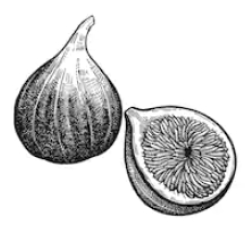
\includegraphics[width=1in,height=1.25in,clip,keepaspectratio]{fig1}}]{Michael Shell}
Use $\backslash${\tt{begin\{IEEEbiography\}}} and then for the 1st argument use $\backslash${\tt{includegraphics}} to declare and link the author photo.
Use the author name as the 3rd argument followed by the biography text.
\end{IEEEbiography}

\vspace{11pt}

\bf{If you will not include a photo:}\vspace{-33pt}
\begin{IEEEbiographynophoto}{John Doe}
Use $\backslash${\tt{begin\{IEEEbiographynophoto\}}} and the author name as the argument followed by the biography text.
\end{IEEEbiographynophoto}

\vfill
\end{document}
